\documentclass{article}

\usepackage[utf8]{inputenc}
\usepackage{hyperref}
\usepackage{amsfonts}
\usepackage{pgfplots}
\usepackage{listings}
\usepackage{tkz-fct}

\title{Lagrange polynomial interpolation over Galois finite fields: A Programmatic Approach}
\author{Alan Cao \\ turingmachine \\
\href{mailto:alan@codemuch.tech}{alan@codemuch.tech}}
\date{January 2018}

\begin{document}

\maketitle

\section{Introduction}

The implementation of mathematical operations in modern computing has become prevalent in many sub-fields and concentration. The power of multi-core processors and random-access memory has enabled high-level programming that can compute complexity in the matter of milliseconds. With the ease of mathematical computation, it is no wonder that modern cryptography has become so integrated with the fields of mathematics, relying on the properties of numbers to create innovative algorithms and cryptosystems. These can range from hashing algorithms, PRNGs, and important secure operations.

This paper aims to examine Lagrange polynomial interpolation at a programmatic approach, rather than one of theory and numerical analysis. Polynomials have been seen to be surprisingly useful and powerful in the fields of computer science, as they display properties that can be applicable to a variety of systems. Polynomial interpolation is one of them, where deconstructed points of a polynomial on a Cartesian \textit{xy}-coordinate plan can be used to reconstruct the original polynomial. 
Joseph-Louis Lagrange's approach will be the main focus of this paper, as it provides us an efficient approach when implemented even in high-level programming languages.

When expressing mathematical concepts such as polynomials, one often thinks about operations with rational numbers, in the field of $\mathbb{Q}$. However, rather than using conventional infinite number sets, we will be introducing the concept of \textit{Galois finite fields} instead. As seen later in \textbf{Section 2}, several restrictions are placed on Lagrange polynomial interpolation, and Galois finite fields will be used to lift them.

In the context of computational complexity in relation to cryptography, it is always important to consider the efficiency of computer algorithms. This is often measured through \textit{time}, where the faster an operation is, the better it becomes. As mentioned above, modern computation have already yielded fast and abstracted\footnote{referring to the high-level of abstractions placed on top of programs and computational operations}. This means that even if an algorithm has been implemented to be much slower and inefficient, it would still be indifferent for users. However, when placing it in the context of cryptography in a modern age of powerful machines, this becomes critical for security and usability. For example, key-distribution servers for large-scale websites must be able to use the quickest and most efficient computational operations to process authentication requests, whether it be sign-ups (key creation) sign-outs (key storage) and logging in (key integrity and validity authentication).

With that said, one important factor to consider is the usage of low-level and systems programming languages, in this case, C for computational operations. C is a programming language that works  with userspace system calls that directly interact with kernelspace, placing it at the near-bottom of the programming language abstraction hierarchy. Since C provides important features such as rapid compilation time and native bitwise operations, it will be utilized throughout the paper.

\section{Lagrange Polynomial Interpolation}

Lagrange polynomial interpolation is defined as a technique of reconstructing a polynomial by utilizing derived points of a Cartesian \textit{xy}-coordinate plane. This process involves the creation of \textit{Lagrange polynomials}, which is represented by this formal theorem:

$$
l_j(x) := \prod_{0\leq m\leq k} \frac{x - x_m}{x_j - x_m} = \frac{x - x_0}{x_j - x_0}...\frac{x - x_{j-1}}{x_j - {x_j}-1} * \frac{x - x_{j+1}}{x_j - x_{j+1}}...\frac{x - x_k}{x_j - x_k}
$$

where $m \neq j$ and $0 \leq j \leq k$. \\

Let's examine the process that it takes for a polynomial to be destructed into points, and then constructed through Lagrange interpolation. 

\subsection{Create data points}

The polynomial to be constructed:

$$
f(x) := 2x^2 + 5x + 8
$$

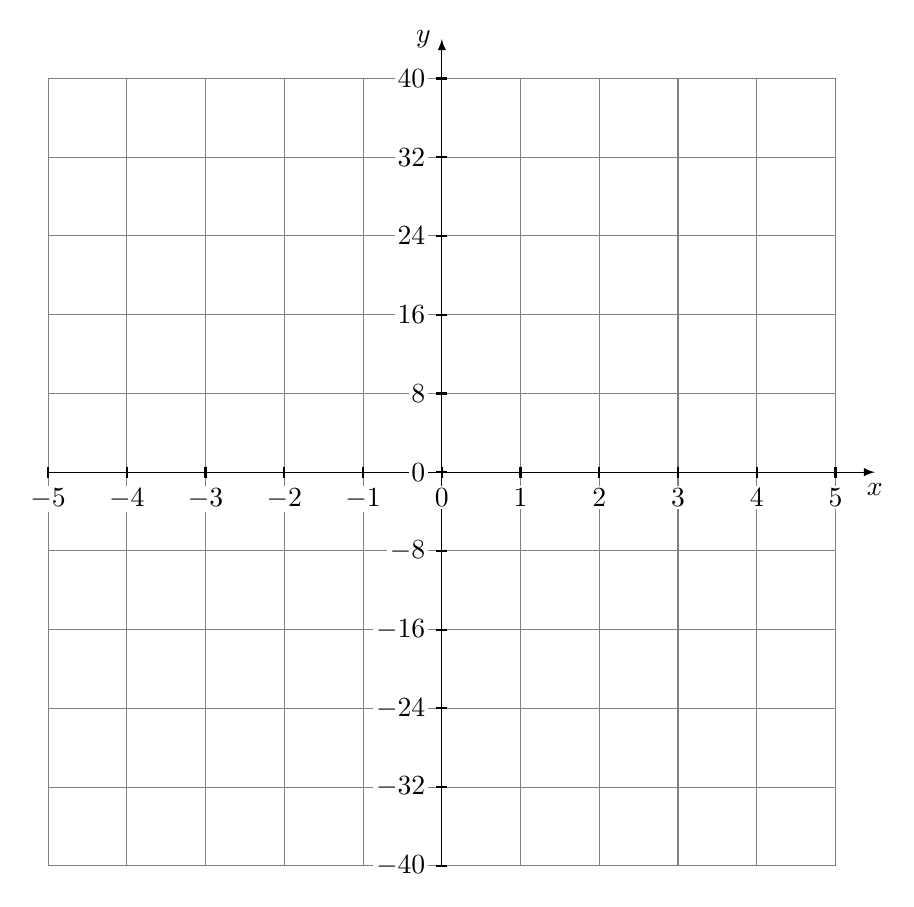
\begin{tikzpicture}
  \tkzInit[xmin=-5,xmax=5,ymin=-40,ymax=40,ystep=8]   
  \tkzGrid
  \tkzAxeXY
  \tkzFct[color=blue,thick,domain = -5:5]{2*x**2+5*x+8};
\end{tikzpicture}
\\
\caption{\textbf{Figure 1.} A graph of polynomial $2x^2 + 5x + 8$}
\\\\
Since the polynomial possesses a degree \textit{d} of 2, it will require $d + 1$, or 3 data points for reconstruction. Data points are selected, where $x \neq 0$. Notice that that the \textit{y} value for $x=0$ is the constant for the polynomial, and therefore cannot be used.

$$
[(1, 15), (2, 26), (3, 41)]
$$

\subsection{Create Lagrange Polynomial}

By using our defined theorem and our constructed data points, we can figure out the coefficients

TODO

\section{Galois Finite Fields}

TODO

\section{Programmatic Implementation}

Now, let's create an implementation of polynomial interpolation over $Gf(2^8)$, or $Gf(256)$.

The first step is creating a preemptive validation function, where the coefficients of a polynomial and $x$-values are passed as arrays. The degree is determined, the polynomial is constructed, and for each supplied $x$-value, a $y$-value is calculated and returned along with it.

\begin{lstlisting}

#include <stdio.h>
#include <stdlib.h>
#include <stdint.h>

typedef uint8_t u8;

typedef struct {
    u8[] coefficients;
    u8[] xvalues;
} lagrange_t;




\end{lstlisting}

\end{document}
